\subsection{Введение в теорию информации.}

информация $=$ - неопределенность - сказал дяденька Шеннон

Для осознания нам поможет рисунок АС:
\begin{center}
    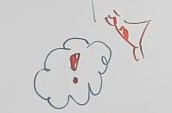
\includegraphics[width = 5cm]{assets/4_1_1.jpg}
\end{center}
Есть что-то - неизвестное - облачко. Затем, вы с помощью глаза заглядываете туда, и ваша неопределенность уменьшается. Соответственно вы получили информацию. То есть сначала была неопределенность $H_1$, потом $H_2$.  $I = H_1-H_2$, откуда и получается наша формула. У него есть глубокий смысл, но создается вопрос: \flqq И че? И что это за неопределенность?\frqq

Ну наличие глаза мешает, непонятно, фу фу фу. Поэтому хотим ввести что-то более формальное и менее абстрактное.

Пусть у нас есть какой-то случайный эксперимент $\Omega$, с вероятностями $p_1,\ldots, p_n$. И вот мы получили информацию что выпало (например орел на монетке).

\deff{Случайный источник} --- черный ящик с красной кнопкой, который показывает номер эл. исхода, когда вы нажимаете на красную кнопку.

Возьмем монетку. Кинули, получили 0 или 1. Теперь возьмем кубик, получим число от 1 до 6. Когда мы кидаем кубик, мы получаем больше информации. И вот Шеннон решил систематизировать все это...

\subsection{Энтропия}

Пусть у нас есть случайный источник и вероятности $p_1,p_2,\ldots ,p_n$. Мы хотим померить численно сколько информации содержится в одном эксперименте:
$$H(p_1,\ldots,p_n):RS\rightarrow R^+$$ 
\deff{Энтропия Шеннона}($H$) - это мера неопределенности или случайности, связанная с случайной переменной. Она измеряет среднее количество информации, необходимое для описания результата случайной переменной. Иными словами, энтропия показывает, насколько непредсказуемым является источник информации.

Возьму пример $p_i = \cfrac{1}{n}$. Введем новое обозначение:
$$h(n) = H\left(\cfrac{1}{n},\cfrac{1}{n},\ldots,\cfrac{1}{n}\right)$$
Очевидно, что $h(n+1)>h(n)$.

Теперь рассмотрим вероятностное пространство и источник на нем:
$$\Omega = \{(1,1),(1,1),\ldots,(1,m_1),(2,1),\ldots,(k,1),\ldots,(k,m_k)\}$$
И давайте теперь каждому причислим какую-то $q_{ij}$, так, что в сумме 1. $p_i = \sum\limits_{j=1}^{m_i}q_{ij}$. Пусть наш случайный источник сломан и показывает  только одно число. Если я возьму сломанный случайный источник от $\Omega$, то мы получим столько же информации сколько и у случайного источника сделанного из $p$. 

Теперь давайте делить это на 2 части. Что вот мы сначала видим первую часть информации, а потом хоба и видим вторую часть информации. И того мы получаем, что когда мы открываем вторую часть мы получим $p_i H(\frac{q_{i1}}{p_i},\ldots, \frac{q_{mi}}{p_i} )$ информации. Откуда благодаря таким рассуждение получаем свойство, которое называется \deff{аддитивностью энтропии}:
$$H(p_1,\ldots,p_k)+\sum\limits_{i=1}^kp_iH(\frac{q_{i1}}{p_i},\ldots, \frac{q_{mi}}{p_i}) = H(q_{11},\ldots, q_{mk})$$

Также для фиксированного $n$, $H$ непр из $\mathbb{R}^n\rightarrow \mathbb{R}$. 



\thmm{Теорема.(Формула энтропии Шеннона)}
$$H(p_1,\ldots,p_n)=-\alpha\sum\limits_{i=1}^np_i\log_2 p_i$$
$\alpha$ отвечает за выбор единицы измерений.

\textbf{Доказательство:}

\thmm{Лемма 1.} $h(n\cdot m) =h(n) + h(m)$.
\begin{quote}
     \textbf{Доказательство:}

     Возьмем  $k=n, m_i=m,p_ = \frac{1}{n},q_{ij} = \frac{1}{nm}$. Из утверждения сверху это верно!
     
\hfill Q.E.D.
\end{quote}
Фиксируем $h(2)=\alpha$. Тогда:

\thmm{Лемма 2.}  $h(2^k)=k\alpha$. тривиально из Леммы 1.

\thmm{Лемма 2,5.}  $h(n^r)=rh(n)$. тривиально из Леммы 1.

\thmm{Лемма 3.} $h(n) = \alpha \log_2n $
\begin{quote}
 \textbf{Доказательство:}

 Найду $i$ такое, что $2^i\leq n^r <2^{i+1}$, где $r\in \mathbb{N}$.
 
 Из монотонности $h$ следует: $\alpha i\leq h(n^r) <\alpha (i+1)$. Поэтому:
 $$\alpha i\leq rh(n) <\alpha \quad\Leftrightarrow\quad a\frac{i}{r}\leq h(n)\leq a\frac{i+1}{r}$$
Также мы знаем, что $i\leq r \log_2 n < i+1$. Получим, что:
$$\alpha \cfrac{i}{r}\leq \alpha log_2 n < \alpha \cfrac{i+1}{r}$$
То есть $\forall r :|h(n)-\alpha log_2n|\leq \cfrac{\alpha}{r}$. Откуда, получаем требуемое равенство.
 
 
 \hfill Q.E.D.
\end{quote}

Возвращаемся к доказательству теоремы. Пусть $p_i$ рациональные. Приведем все $p$ к общему знаменателю и пусть теперь $p_i  = \cfrac{a_i}{b_i}$. Возьму $m_i = a_i$, $r_{ij}=\cfrac{1}{a_i}, q_{ij} = \cfrac{1}{n}$. Подставим во второе неравенство получим:
$$H\left(\cfrac{1}{b},\cfrac{1}{b},\ldots, \cfrac{1}{b}\right)= H(p_1,p_2,\ldots,p_k) + \sum\limits_{i=1}^kp_i H\left(\cfrac{1}{a_i},\ldots,\cfrac{1}{a_i}\right)$$
Что тут происходит? Я разбиваю каждый исход изначальный, на $a_i$ исходов по $\frac{1}{b_i}$. С одной стороны я получаю $b$ исходов по $\frac{1}{b}$. С другой стороны я могу выбрать исход, а потом его разбить. Откуда по аддитивности и получается такая формула. А она в свою очередь уже удобная, так как в ней повторяются значения внутри $H$, так что можем заменить на $h$:
$$h(b) = H(p_1,\ldots,p_k)+\sum\limits_{i=1}^kp_ih(a_i)$$
Заметим, что $\sum\limits_{i=1}^np_i=1$, так что левую часть на эту сумму:
$$\sum\limits_{i=1}^np_ih(b) = H(p_1,\ldots,p_k)+\sum\limits_{i=1}^kp_ih(a_i)$$
$$H(p_1,\ldots,p_k)=\sum\limits_{i=1}^np_i(h(b)-h(a_i))$$
$$H(p_1,\ldots,p_k)=\sum\limits_{i=1}^np_i(\alpha log_2b-\alpha log_2a_i) = -\alpha\sum\limits_{i=1}^np_i\log_2 p_i$$
Эта формула верна и не для рац. исходя непрерывности (любое не рац. можно зажать с двух сторон сходящимися последовательностями и мы победили)

\hfill Q.E.D.

$\alpha$ --- бит, единица информации.

Обычно используется логарифм по основанию 2, тогда энтропия измеряется в битах (или "Шеннонах"). Если используется натуральный логарифм (основание e), то энтропия измеряется в натах. Использование логарифма по основанию 10 даёт единицы измерения в децитах (Hartleys). Выбор основания влияет только на масштаб энтропии, а не на её относительные значения.

Энтропия Шеннона имеет широкое применение в различных областях, включая:

\begin{itemize}
    \item Теория информации: Является фундаментальным понятием для измерения количества информации.
    \item Сжатие данных: Используется для оценки теоретического предела сжатия данных.
    \item Криптография: Оценка случайности ключей и стойкости шифров.
    \item Машинное обучение: В деревьях решений используется для выбора признаков, которые лучше всего разделяют данные.
    \item Обработка естественного языка (NLP): Оценка неопределенности в языковых моделях.
    \item Термодинамика: Аналогична термодинамической энтропии, отражает меру беспорядка в системе.
\end{itemize}

Также есть такие понятия, как взаимная энтропия и условная энтропия. Их определения появятся в конспекте после того, как пройдет неделя со сдачей домашки.
